\section{CartPole}
\subsection{Transition Distribution By Angle}
\begin{figure}[h!]
	\centering
	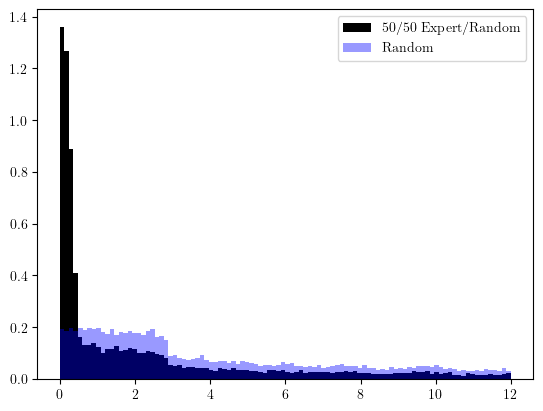
\includegraphics[width=\textwidth]{Figures/angles_cp.png}
	\caption{Histogram plot of transitions initial state against absolute angle. 50/50 Expert/Random refers to the joint expert-random dataset. }
	\label{ap:dist_cp}
\end{figure}

\subsection{Supervised-Dyna}

\begin{figure}[h!]
	\centering
	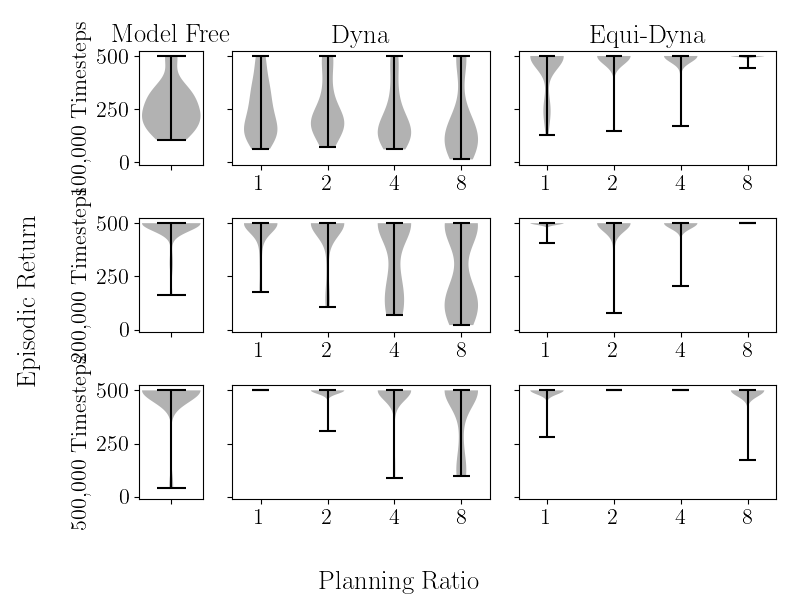
\includegraphics[width=\textwidth]{Figures/violin_cp_expert.png}
	\caption{Violin Plot of episodic returns at timestep intervals across all tested planning ratios on the CartPole environment.}
\end{figure}

\begin{figure}[h!]
	\centering
	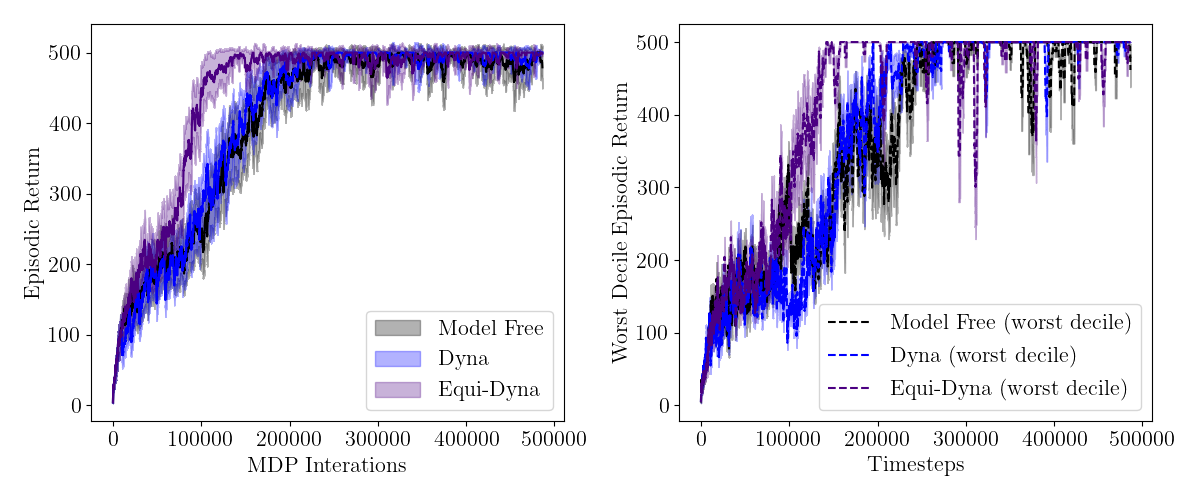
\includegraphics[width=\textwidth]{Figures/Expert_dyna_cp_pr1.png}
	\caption{Episodic returns for Supervised-Dyna agents with a baseline on the CartPole environment. Using a planning ratio of one.}
\end{figure}
\begin{figure}[h!]
	\centering
	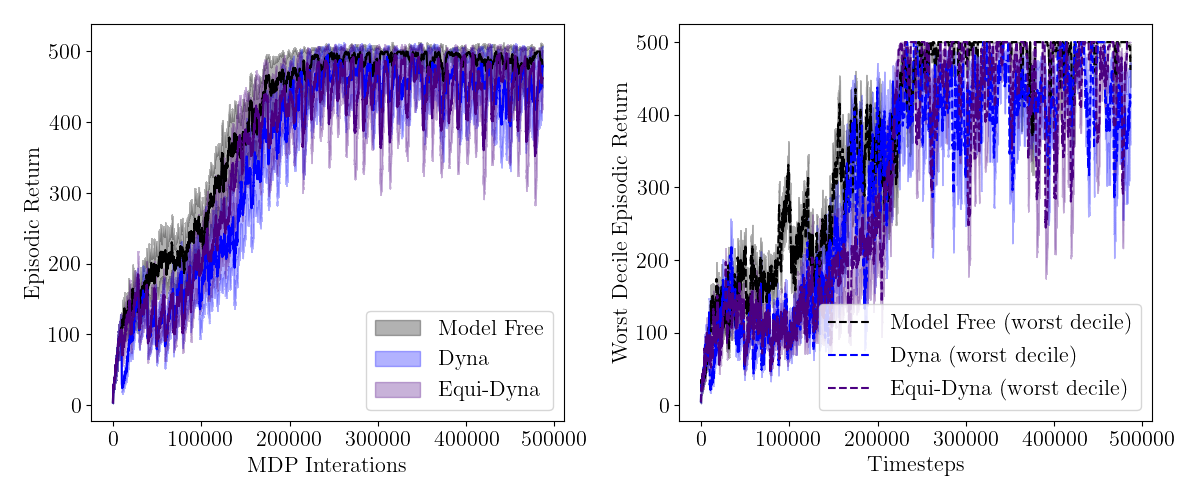
\includegraphics[width=\textwidth]{Figures/Expert_dyna_cp_pr2.png}
	\caption{Episodic returns for Supervised-Dyna agents with a baseline on the CartPole environment. Using a planning ratio of two.}
\end{figure}
\begin{figure}[h!]
	\centering
	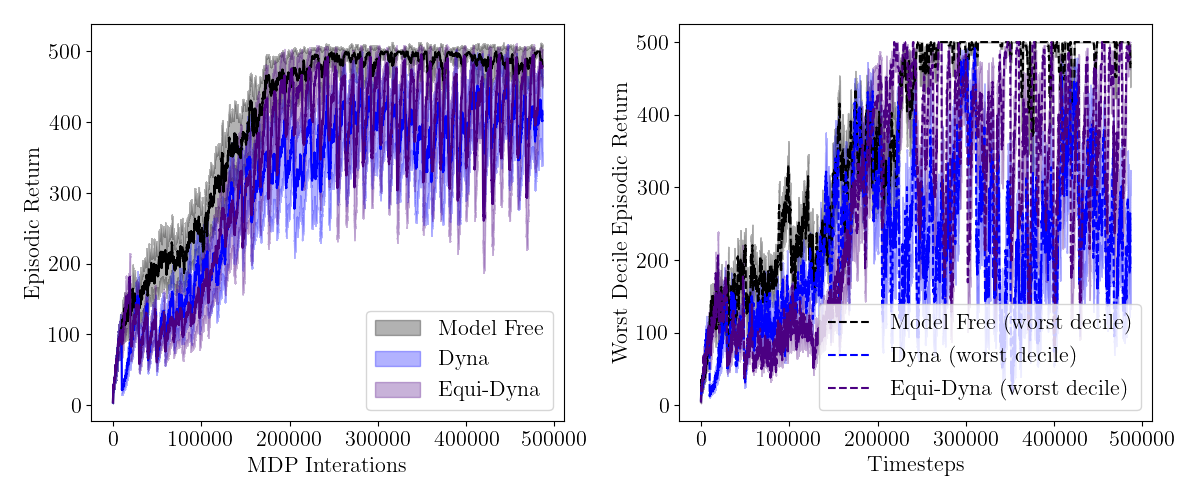
\includegraphics[width=\textwidth]{Figures/Expert_dyna_cp_pr4.png}
	\caption{Episodic returns for Supervised-Dyna agents with a baseline on the CartPole environment. Using a planning ratio of four.}
\end{figure}
\begin{figure}[h!]
	\centering
	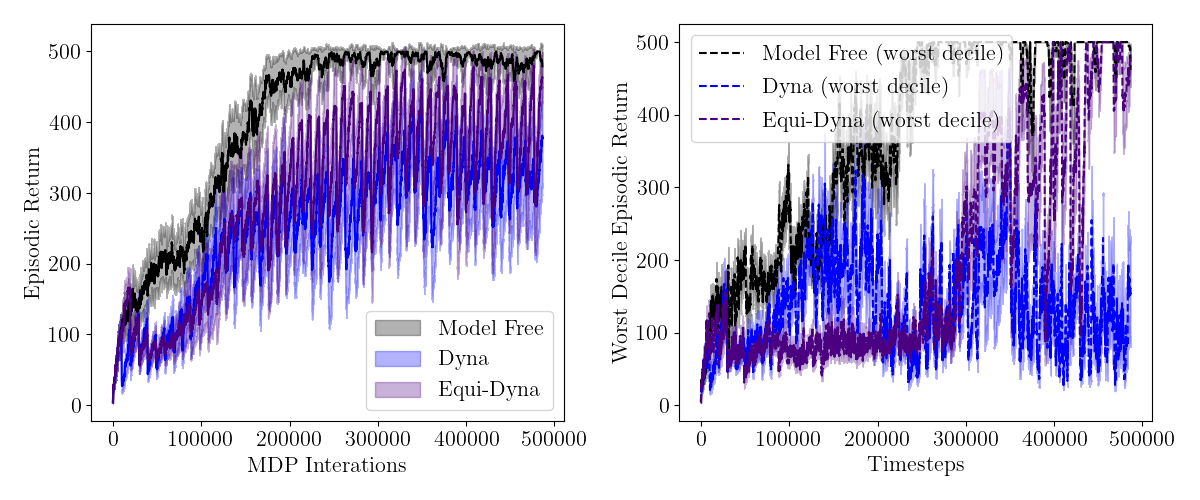
\includegraphics[width=\textwidth]{Figures/Expert_dyna_cp_pr8.png}
	\caption{Episodic returns for Supervised-Dyna agents with a baseline on the CartPole environment. Using a planning ratio of eight.}
\end{figure}

\newpage

\section{Catch}



\subsection{Supervised-Dyna}\label{ap:supervised-dyna-catch}

\begin{figure}[h!]
	\centering
	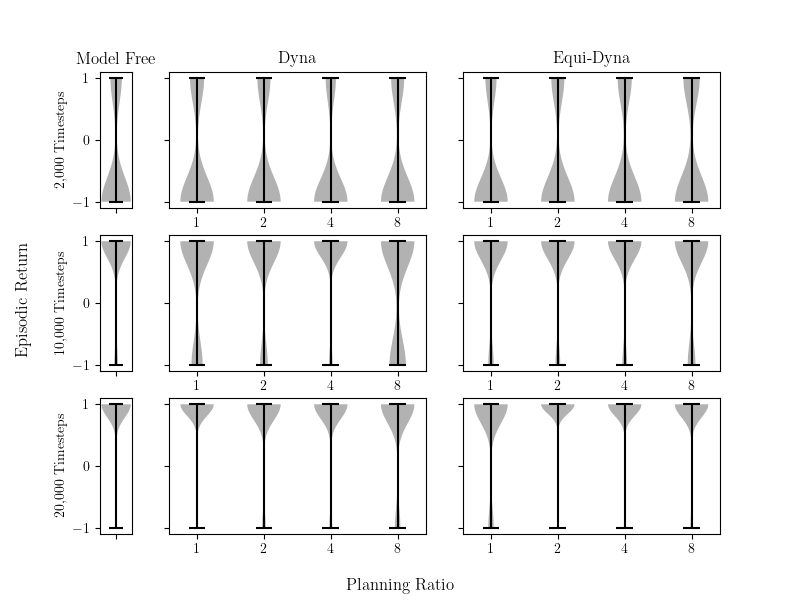
\includegraphics[width=\textwidth]{Figures/violin_catch_expert.png}
	\caption{Violin Plot of episodic returns at timestep intervals across all tested planning ratios on the catch environment.}
\end{figure}

\begin{figure}[h!]
	\centering
	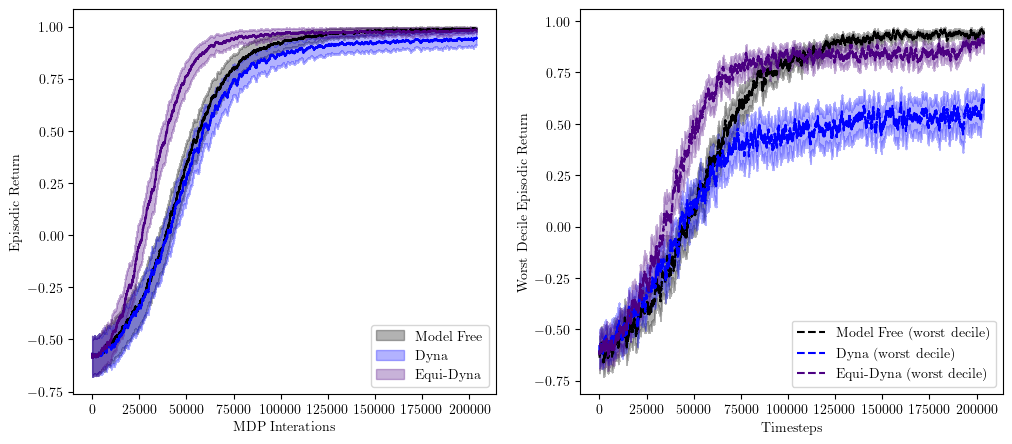
\includegraphics[width=\textwidth]{Figures/Expert_Dyna_Catch_pr1.png}
	\caption{Episodic returns for Supervised-Dyna agents with a baseline on the Catch environment. Using a planning ratio of one.}
\end{figure}
\begin{figure}[h!]
	\centering
	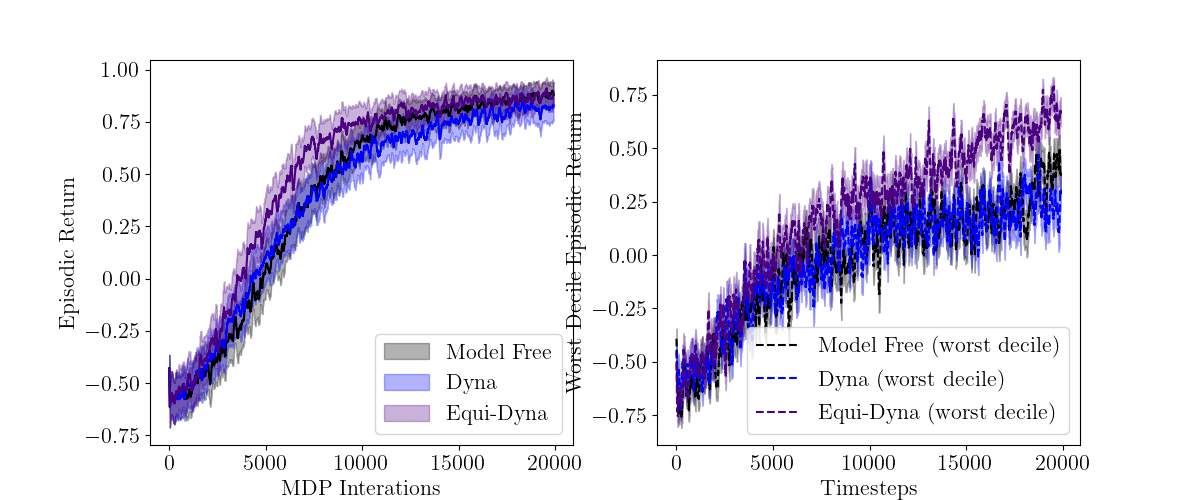
\includegraphics[width=\textwidth]{Figures/Expert_Dyna_Catch_pr2.png}
	\caption{Episodic returns for Supervised-Dyna agents with a baseline on the Catch environment. Using a planning ratio of two.}
\end{figure}
\begin{figure}[h!]
	\centering
	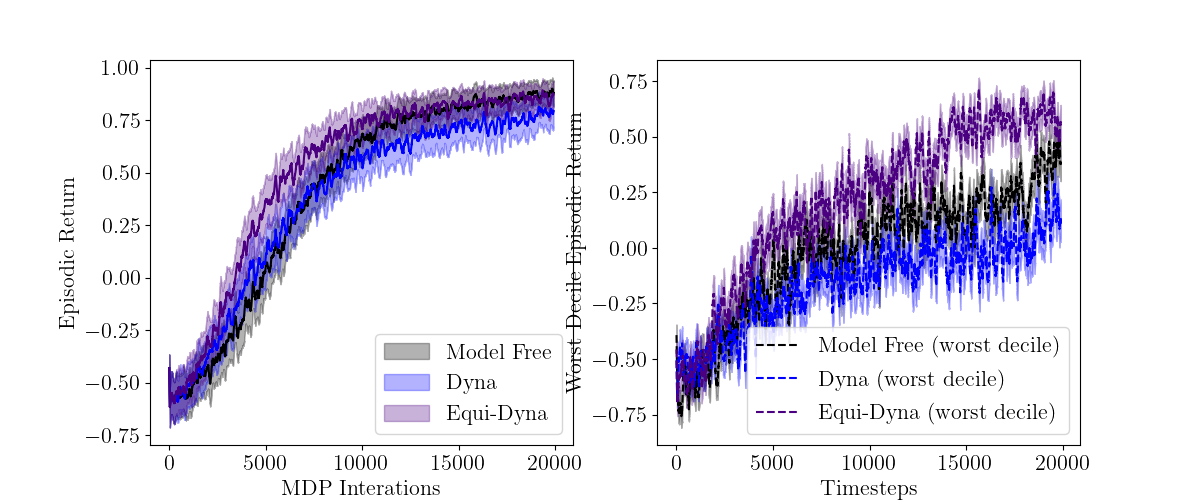
\includegraphics[width=\textwidth]{Figures/Expert_Dyna_Catch_pr4.png}
	\caption{Episodic returns for Supervised-Dyna agents with a baseline on the Catch environment. Using a planning ratio of four.}
\end{figure}
\begin{figure}[h!]
	\centering
	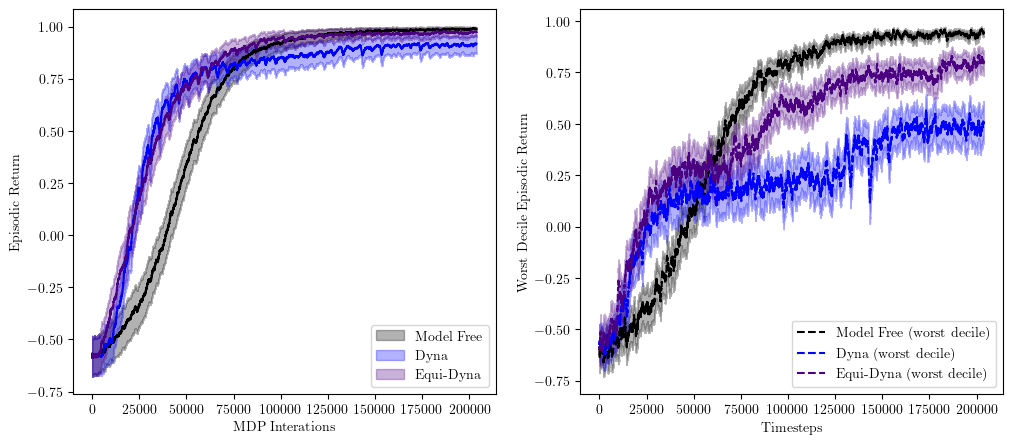
\includegraphics[width=\textwidth]{Figures/Expert_Dyna_Catch_pr8.png}
	\caption{Episodic returns for Supervised-Dyna agents with a baseline on the Catch environment. Using a planning ratio of eight.}
\end{figure}
